% E.1 矩形 OABC，A(6,0), C(0,4), B(6,4). P 沿 O→A→B, Q 沿 C→B
% 示例时刻 t=2: P(4,0), Q(2,4)
\documentclass[tikz,border=4pt]{standalone}
\usepackage{ctex}
\usepackage{amsmath}
\usetikzlibrary{calc, arrows.meta}
\begin{document}
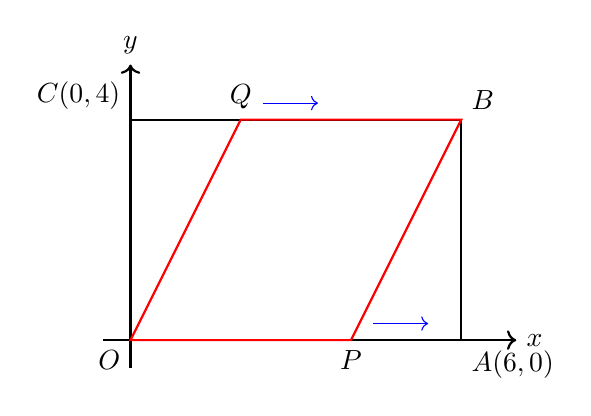
\begin{tikzpicture}[scale=0.7, thick]
  \coordinate (O) at (0,0);
  \coordinate (A) at (6,0);
  \coordinate (B) at (6,4);
  \coordinate (C) at (0,4);
  \coordinate (P) at (4,0);
  \coordinate (Q) at (2,4);

  % 坐标轴
  \draw[->] (-0.5,0) -- (7,0) node[right]{$x$};
  \draw[->] (0,-0.5) -- (0,5) node[above]{$y$};

  \draw (O)--(A)--(B)--(C)--cycle;
  \draw[red, thick] (O)--(P)--(B)--(Q)--cycle;

  \draw[->, blue, thin] (4.4,0.3) -- (5.4,0.3);
  \draw[->, blue, thin] (2.4,4.3) -- (3.4,4.3);

  \node[below left] at (O) {$O$};
  \node[below right] at (A) {$A(6,0)$};
  \node[above right] at (B) {$B$};
  \node[above left] at (C) {$C(0,4)$};
  \node[below] at (P) {$P$};
  \node[above] at (Q) {$Q$};
\end{tikzpicture}
\end{document}
